Mechanics is a discipline that analyzes and simplifies physical systems to solve a wide range of problems, from everyday challenges to complex engineering applications. Assumptions are not bad, but they have to be plausible!
\begin{figure}[H]
	\begin{center}
		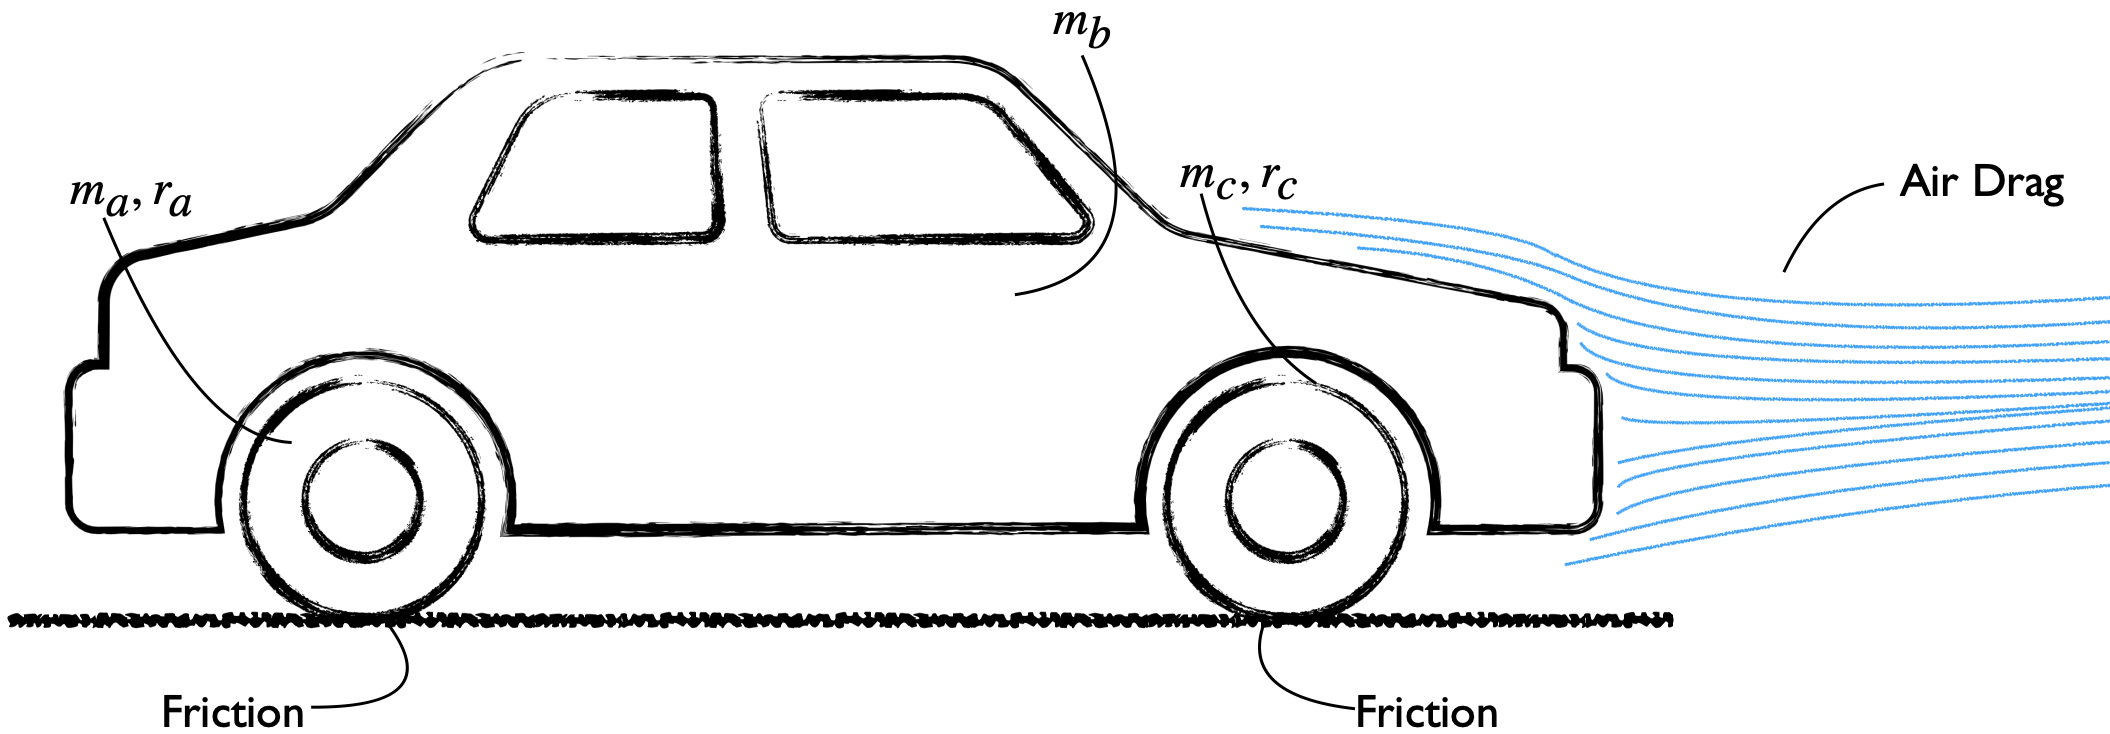
\includegraphics[width=\linewidth]{car.png}
	\end{center}
	\caption{Simplified Car Dynamics Model with Resistive Forces}
	\label{fig: model}
\end{figure}
	Figure \ref{fig: model} shows the system of a car ready to start the testing. There is the main body, two wheels (for now indexed as wheel $a$ and $c$) and dissipative forces, i.e. the drag resistance and friction, slowing the vehicle down. We omit the spring and damper in the vehicle dynamics model, as we focus solely on longitudinal behavior and assume a rigid body.
\begin{figure}[H]
	\begin{center}
		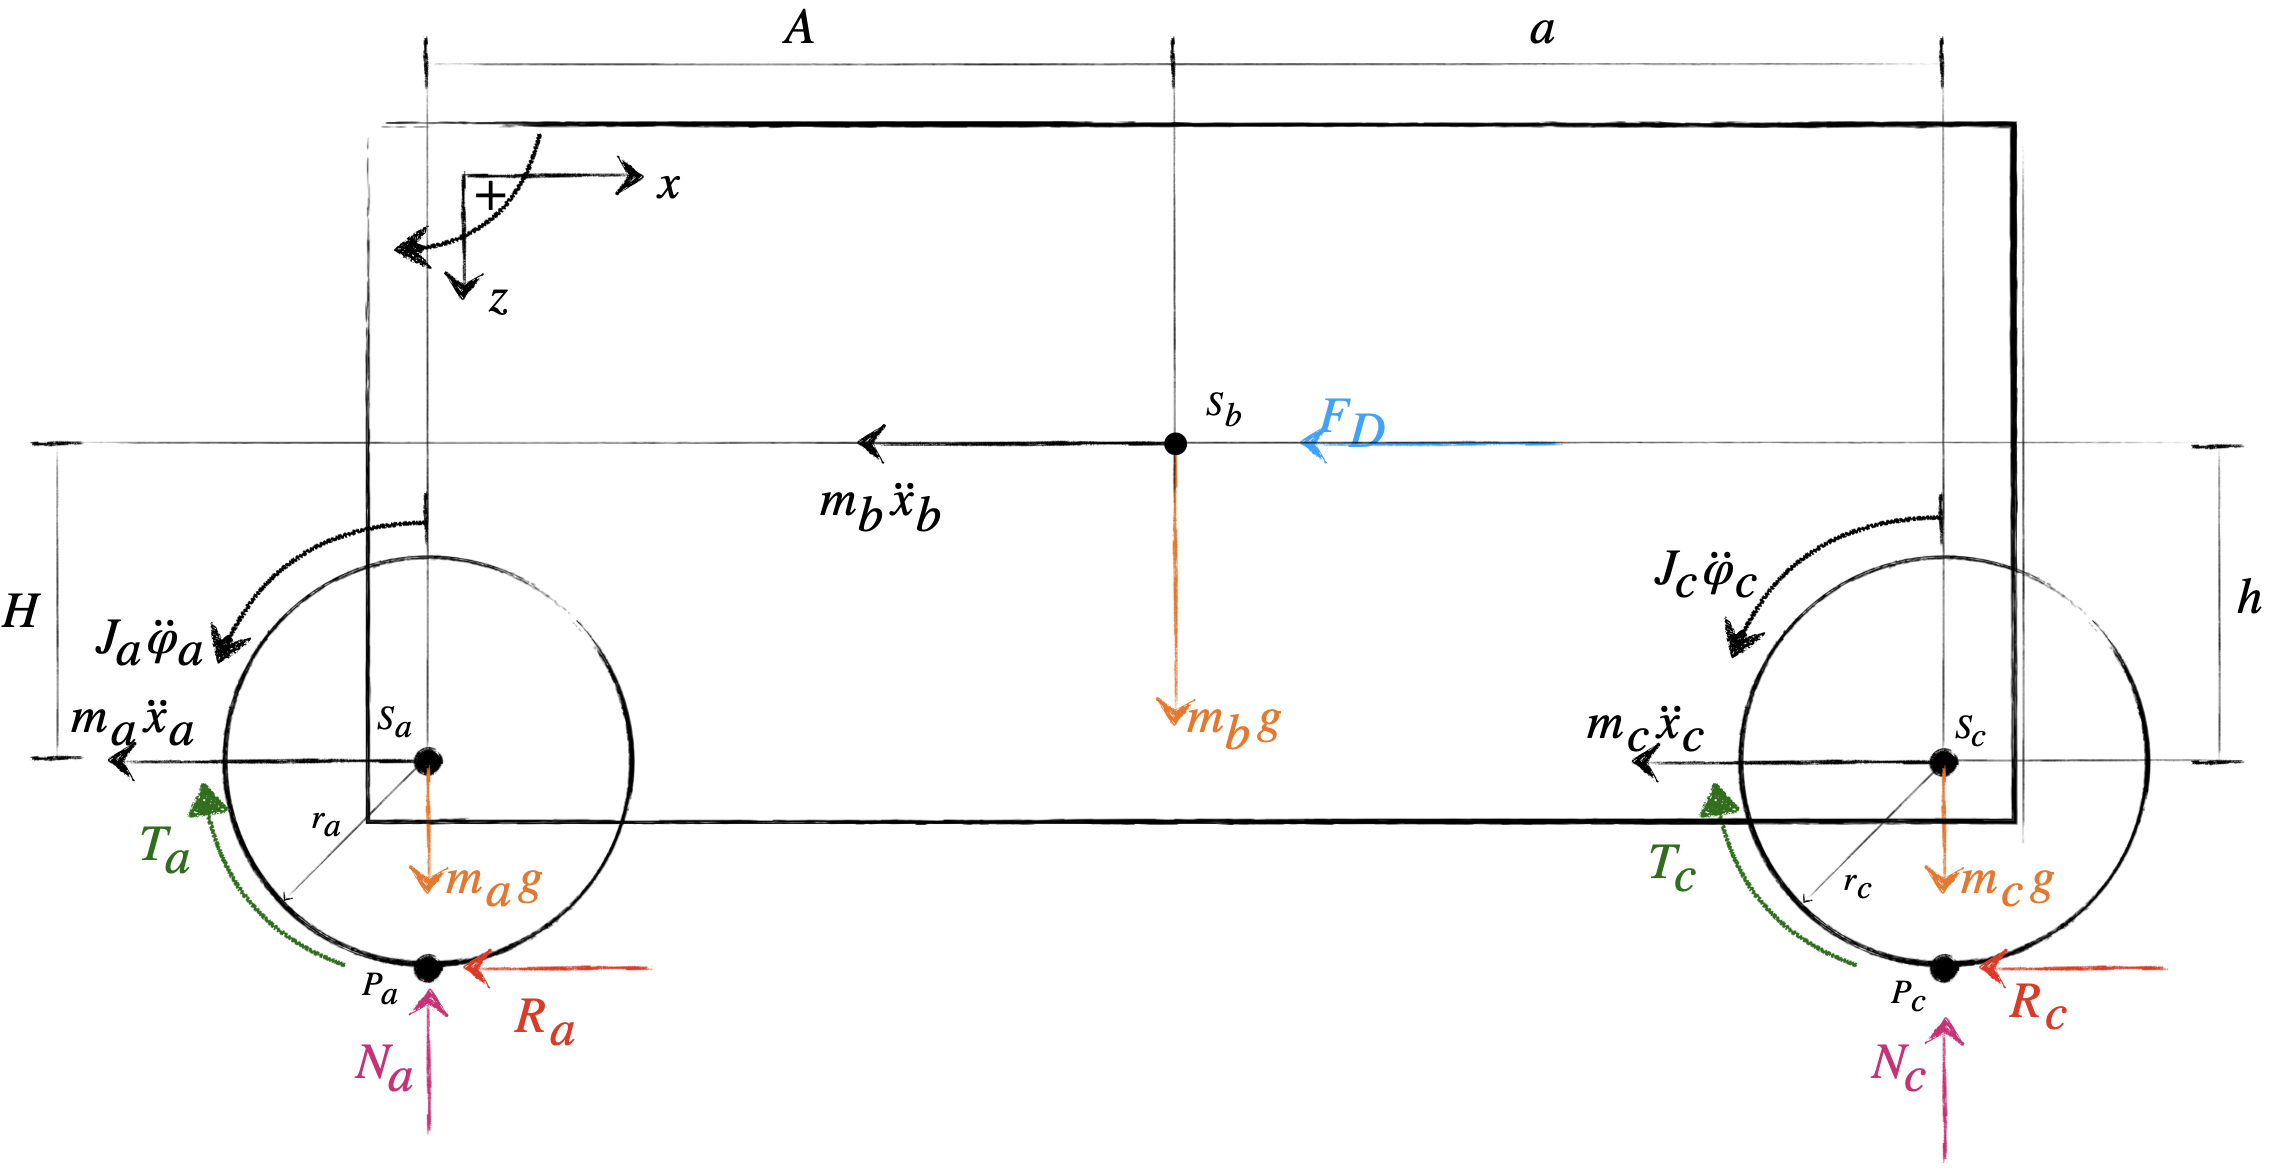
\includegraphics[width=\linewidth]{whole.png}
	\end{center}
	\caption{Forces Acting on the Vehicle \\(d'Alembert's Principle)}
	\label{fig: forces}
\end{figure}
Figure \ref{fig: forces} depicts a 2D model of a simplified car dynamics system. The objective is to derive a differential equation of motion for the vehicle, from which the Tractive Force can be expressed in the form of:
\begin{equation*}
	F(t) = A + B\dot x + C\dot x^2 + D\ddot x.
\end{equation*}
In this section, we focus on the most critical components contributing to the vehicle's motion:  \textit{Tractive Force}, \textit{Rolling Resistance}, \textit{Aerodynamic Drag} and \textit{Types of Wheel Drives}. The complete derivation of the equations is included in \ref{sec: apx} Appendix.
\subsubsection*{Tractive Force}
	The tractive force $F_T$ is the force that propels a vehicle forward by generating motion at the tire–ground interface. It is related to the torque at the wheel $T$ through:
	\begin{equation*}
		T = F_T\cdot r,
	\end{equation*}
	where $r$ is the effective rolling radius of the tire. This relation assumes an idealized system without drivetrain losses; efficiency factors and gear ratios are incorporated in later sections.
\subsubsection*{Rolling Resistance}
	The rolling resistance force $R$ arises from the interaction between the tire and the ground, primarily due to the deformation of both the tire and the surface. When the engine applies torque to the wheels, resulting in a tractive force at the contact patch, rolling resistance is present. It is commonly modeled as
	\begin{equation*}
		R = c_R N,
	\end{equation*}
	where $c_R$ is the rolling resistance coefficient and $N$ the normal force. For our analysis, we adopt the value for the coefficient of $0.12$, as the findings of \parencite{wargula2019determination} indicated this value as the most recurrent for motor vehicles with pneumatic tires on asphalt/concrete surfaces.
	\begin{equation*}
		c_R = 0.12
	\end{equation*}
	
\subsubsection*{Aerodynamic Drag}
	The drag force air-resistance is given by: 
	\begin{equation*}
		F_D(v) = \frac{1}{2}\rho_a c_D A_F v^2,
	\end{equation*}
	where $\rho_a$ is the specific air density, $c_D$ is the drag coefficient, $A_F$ is the effective frontal area $A_F$ and $v$ is the relative velocity. The Drag Coefficient $c_D$ and Frontal Area $A_F$ depend on the shape and aerodynamic properties of the vehicle.
	
	The air density $\rho_A$ depends on the ambient conditions and can be approximated by 
	\begin{equation*}
		\rho_a = \frac{0.0348p}{T},
	\end{equation*}
	where $p$ is the atmosphere pressure and $T$ - the temperature. For standard conditions ($p= 1$ bar and $T= 15\degree C=288.15K$), this yields an air density of $1.225kg/m^3$ \parencite[p. 135]{mashadi2012vehicle}. 
	
	Since velocity is the time derivative of position, i.e. $v=\dot x$, the drag force can also be expressed as:
	\begin{equation*}
    	F_D = \frac{1}{2}\rho_a c_D A_F \dot x^2.
	\end{equation*}

\subsubsection*{Wheel Drive Types}
	Vehicles can be equipped with either all-wheel drive (AWD) or two-wheel drive (TWD) systems, the latter being subdivided into front-wheel drive (FWD) and rear-wheel drive (RWD). Our model assumes an AWD configuration. Why is this important? Because the number and position of driven wheels directly influence the distribution of tractive force and frictional load across the tires.
	
	In TWD systems, only two wheels receive torque. In FWD vehicles, the front tires are responsible for both steering and propulsion, which can lead to understeering behavior under heavy acceleration. In contrast, RWD vehicles transmit torque through the rear wheels, often offering better weight distribution during acceleration but less traction on slippery surfaces.
	
	From a modeling perspective, non-driven wheels do not contribute to propulsion and thus experience no tractive friction. They primarily support the vehicle's weight and may generate rolling resistance. In AWD systems, torque is distributed across all wheels, which changes how forces—particularly tractive and rolling resistances—are shared among the tires. This impacts the overall force balance and must be accounted for in the dynamics.
	
\subsubsection*{Differential Equation of Motion}
	Each of the AWD, RWD and FWD have different equations of motion.
	
	Differential equation of motion for RWD vehicles:
	\begin{align*}
		\begin{split}
			F_{T,RWD} = \frac{5\cdot\frac{2m_a + m_b}{2 + \frac{h}{a}c_R}c_Rg}{2 + \frac{5c_Rr_a}{2a+hc_R}} & + \frac{3\rho_a c_D A_F}{4 + \frac{10c_Rr_a}{2a+hc_R}}\dot x^2 \\
				& + \frac{3m_b - 5\cdot\frac{m_c+m_a}{2a + hc_R}c_Rh}{{2 + \frac{5c_Rr_a}{2a+hc_R}}}\ddot x
		\end{split}
	\end{align*}
	Differential equation of motion for FWD vehicles:
	\begin{align*}
		F_{T,FWD} = \frac{ 5\cdot\frac{2m_c + m_b}{2 - \frac{h}{a}c_R}c_Rg}{2 - \frac{5c_Rr_c}{2a-hc_R}} &  + \frac{3\rho_a c_D A_F}{4 - \frac{10c_Rr_c}{2a-hc_R}}\dot x^2 \\
			& + \frac{3m_b + 5\cdot\frac{m_c+m_a}{2a - hc_R}c_Rh}{2 - 5\cdot\frac{c_Rr_c}{2a-hc_R}}\ddot x 
	\end{align*}
	Differential equation of motion for AWD vehicles:
	\begin{align*}
		F_{T,AWD} & = \frac{5}{4}c_Rmg  + \frac{3}{8}\rho_a c_D A_F \dot x^2 + \frac{3}{4}m_b\ddot x
	\end{align*}